\documentclass[a4paper]{book}
\usepackage{extarrows}
\usepackage{amsmath,amsthm}
\usepackage{amsmath}
\usepackage{amssymb}
\usepackage{amsfonts}
\usepackage{answers}
\usepackage{eufrak}
\usepackage{eucal}
\usepackage{fancyhdr}
\usepackage{graphicx}
{\setlength\arraycolsep{2pt}
\usepackage{mathrsfs}
\usepackage{graphicx,fancyhdr}
\usepackage{graphicx} 
\graphicspath{ {./images/} }
\usepackage{CJKnumb}
\usepackage{titlesec}
\titleformat{\chapter}{}{}{0em}{\bf\huge}
\usepackage{amsthm}
\usepackage{cite}
\usepackage[utf8]{inputenc}
\usepackage[colorlinks,urlcolor=blue,citecolor=blue,linkcolor=blue]{hyperref}
\usepackage{tikz}
\usepackage{setspace}
\usepackage{xspace}
\usepackage{cite}

\newtheorem{theorem}{Theorem}%[section]
\newtheorem{lemma}[theorem]{Lemma}%[section]
\newtheorem{example}{Example}%[section]
\newtheorem*{remark*}{Remark}%[section]
\newtheorem*{note*}{Note}%[section]
\newtheorem{proposition}{Proposition}%[section]
\newtheorem{definition}{Definition}%[section]
\newtheorem{conjecture}{Conjecture}%[section]
\newtheorem{corollary}{Corollary}%[section]
\newtheorem{problem}{Problem}%[section]
\newtheorem{condition}{Condition}%[section]

\renewcommand{\proofname}{\textbf{Proof}}

\newenvironment{ddd}{\begin{rmdef}\rm}{\end{rmdef}}                             
\newenvironment{eee}{\begin{rmexa}\rm}{\end{rmexa}}                             
\newenvironment{rrr}{\begin{rmrem}\rm}{\end{rmrem}}                                   
					                                        
\newenvironment{pf}[1][Proof]{\par\noindent{\em #1}. }{\hfill\framebox(6,6)\par\medskip}

\usepackage{geometry}
 \usepackage[normalem]{ulem}
%\renewcommand{\baselinestretch}{1.5}

\geometry{left=3.5cm,right=3.5cm,top=2.5cm,bottom=2.5cm}

\newcommand{\Poincare}{Poincar\'e\xspace}
\newcommand{\Holder}{Hölder}

\usepackage{graphicx} %picture
\usepackage{float} %picture
\usepackage{subfigure} %picture

\usepackage[nottoc,notlot,notlof]{tocbibind}
%Hölder
%\renewcommand{\baselinestretch}{1.5}
\let\cleardoublepage\clearpage
\begin{document}

\begin{titlepage}\phantom{|}\vspace{0.75in}
\begin{center}
    \underline{THE ISOPERIMETRIC PROBLEM}
\end{center}
\begin{center}
    \underline{}
\end{center}
\vspace{1.5in}%{2.0in}
\begin{center}
    Dissertation submitted at the University of Leicester \\
    in partial fulfilment of the requirements for \\ 
    the degree of Bachelor of Science of Mathematics\\
\end{center}
\vspace{.5in}
\begin{center}
    by
\end{center}
\vspace{.5in}
\begin{center}
    Steven Cheung \\
    Department of Mathematics \\
    University of Leicester \\
\end{center}
\vspace{0.5in}
\begin{center}
    May 2024
\end{center}
\end{titlepage}

\tableofcontents
\thispagestyle{empty}
\chapter*{Declaration}                % The * means no number for this chapter
\pagenumbering{arabic}
\addcontentsline{toc}{chapter}{\hspace{0.2in}Declaration}
All sentences or passages quoted in this project dissertation from other
people's work have been specifically acknowledged by clear cross referencing
to author, work and page(s).  I understand that failure to do this amounts
to plagiarism and will be considered grounds for failure in this module and
the degree examination as a whole.


\bigskip

\noindent
Name: Steven Cheung


\bigskip

\noindent
Signed: (add the signature from adobe pdf editor)


\bigskip

\noindent
Date: 


\chapter*{Abstract}
\addcontentsline{toc}{chapter}{\hspace{0.2in}Abstract}
In general, we want the maximum area whose boundary has a specific length. 
\newline
\newline
For the 2-dimensional case.
\newline
\newline
For the 3-dimensional.
\newline
\newline
For the $n$-dimensional.
\newline
\newline
Manifolds?


\chapter*{Introduction}
\addcontentsline{toc}{chapter}{\hspace{0.2in}Introduction}
\section*{Historical Notes}
\addcontentsline{toc}{section}{\hspace{0.2in}Historical Notes}
Isoperimeter, isos which is ancient Greek for equal and perimetron for perimeter. The isoperimetric perimetric problem, even though not properly formalized, was already thought about all throughout the history. 
\newline
\newline
Book V of Pappus of Alexandria's Mathematical collections ~\cite{wiegert2010sagacity} began with a preface titled "On the Sagacity of Bees", rather than the history of mathematicians past or their accomplishments to follow. This was written near the end of the 3rd century $A.D.$. Observing, Pappus credited the bees with "a certain geometrical forethought" (Thomas 593~\cite{ivor1941selections}) for their nearly faultless hexagonal comb structre. He wrote
\begin{center}
    \begin{quote}
        "Bees know just this fact which is useful to them, that 
        the hexagon is greater than the square and the triangle 
        and will hold more honey for the same expenditure of 
        material in constructing each"
    \end{quote}
    (Thomas 593~\cite{ivor1941selections})
\end{center}
Beyond the efficiency of bees, Pappus prefaced, "We" he continued
\begin{center}
    \begin{quote}
        "... will {}investigate a somewhat wider problem, namely that, 
        of all equilateral and equiangular plane figures having an equal 
        perimeter, that which has the greater number of angles is always great 
        and the greates of them all is the circle having it's perimeter equal to them"
    \end{quote}
    (Thomas 593~\cite{ivor1941selections})
\end{center}

Pappus then started working on the isoperimetric problem, which included numerous smaller problems within it. The main objective of the problem is to determine which of the planes and figures with the same perimeter has the largest area amongst them.

Although Pappus addressed the problem in the collections, it has been a topic of interest for centuries before. Appearing in both mathematical and literary materials and captivating the minds of mathematicians. 
\newline
\newline
The isoperimetric issue demonstrates ancient mathmaticians' perceptiveness and the consistency of mathematical endeavor over time, even in the modern age. The isoperimetric problem have been used by poets and historians, despite its mathematical nature. Most famously, Virgil made use of the concept in his Roman epic, The Aeneid. To quote Virgil
\begin{center}
    \begin{quote}
        "At last they landed, where from far your eyes
        May view the turrets of new Carthage rise;
        There bought a space of ground, which Byrsa call'd,
        From the bull's hide they first inclos'd and wall'd.""
    \end{quote}
    (Book I of Aeneid~\cite{virgil1981aeneid})
\end{center}

Virgil's version has it that Dido, daughter of the king of Tyre, fled home after her brother killed her husband. Dido ended up on the north coast of Africa, where she bargained to buy as much land as she could enclose with an oxhide. Thus, she cut the hide into thin strips, presumably met and solved enclosing the largest area with a given perimeter - the isoperimetric problem. Dido may have been clever enough and chose an area by the coast to exploit the shore as part of the perimeter. But this mostly spoils the purity of posed problem. Kline concludes~\cite{kline1985mathematics}. The Aeneid was written between $29$ and $19 B.C.$.
\begin{figure}[h]
    \begin{center}   
        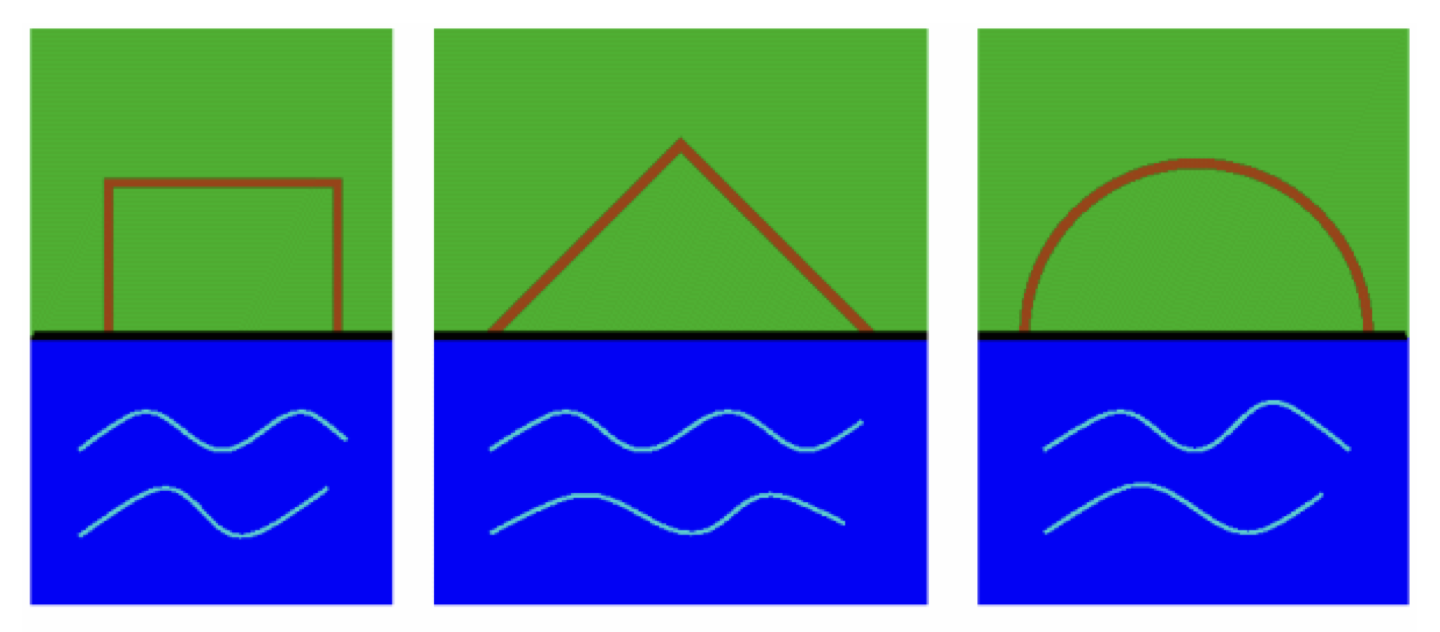
\includegraphics[width=60mm]{dido_1}
        \caption{Representations of areas bounded by common shapes of the same perimeter. The semicircle, answer to Dido's problem which contains the greatest area. (image and caption from~\cite{demjanenko2008isoperimetric})}
    \end{center}
\end{figure}
\leavevmode

In the 3rd century $A.D.$, Roman historian Marcus Junianus Justinus compliled an account of Carthaginian folklore that the legendary founding of Carthage by Dido, called Elissa by the Greeks (the mythological origin of the city):
\begin{center}
    \begin{quote}
        "Then [Elissa] bout some land, just as much as could be covered by a cow's hide, where she could give some recreation to her men... She next gave orders for the hide to be cut into very fine strips, and in this way she took possession of a great area than she had apparently bargained for"
    \end{quote}
    (Book XVIII 157~\cite{yardley1994justin})
\end{center}

So since ancient Greece, around $100B.C.$, they wanted to measure the size of islands by timing how long it takes to circumnavigate the entire island. Proclus, a classical mathematician, mocked geometers for "measuring the size of a city from the lengths of its walls". To the common person of antiquity, two shapes with equal perimeter may have different areas. Interestingly, some individuals exploited this misconception to defraud others of land. Considerably more amusing, these con artists were viewed as liberal which demonstrates how unnatural the idea of shapes with a similar edge having different regions was to the old Greeks.
\newline
\newline
Geoffrey of Monmouth's Historia Regum Britanniae (History of the Kings of England), a 12th century $A.D.$ chronicle of Arthurian legends, mentions the isoperimetric problem. In this story, Hengist, a German duke, appeals to King Vortigern for land in exchange for his military service:
\begin{center}
    \begin{quote}
        "'Grant', said Vortigern, 'unto thy servant but so much only as may be compassed round about by a single thong within the land thou hast given me, that so I ma build me a high place therein whereunto if need be I may betake me’...Straightaway...Hengist took a bull’s hide, and wrought the same into a single thong throughout. He then compassed round with his thong a stony place that he had right cunningly chosen, and within the space thus meted out did begin to build a castle that was afterwards called in British , Kaercorrei, but in Saxon, Thongceaster, the which in Latin’s speech is called Castrum corrigae'"
    \end{quote}
    (Monmouth 105-106~\cite{evans1920histories})
\end{center}
\leavevmode
\newline
\newline
Thus, the poets and historians who chronicled the exploits of these mythological characters as well as the figures themselves found special meaning in the isoperimetric problem. Despite its extensive implications, the notion of isoperimetry was "naturally greek". The Greeks have pretty much solved it, by their standards. Zenodorus was an ancient Greek mathematician from around $200B.C.$ to $120B.C.$. And have mostly proved that a circle has greater area than any polygon with the same perimeter. Majority of his work was lost. However, fortunately, parts of his work survived through references by Pappus and Theon of Alexandria.

Theon of Alexandria then develops this idea, with a summary of the proofs present by Zenodorus in "On Isoperimetric Figures". According to Theon, Zenodorus did not initiate his disussion of isoperimetry with the circle. Rather he stated that "Of all rectilinear figures having an equal perimeter - I mean equilateral and equiangular figures - the greatest is that which has the most angles" (Thomas 388-389~\cite{ivor1941selections}). In more modern language, the proposition is stated as follows: "Given two regular $n$-gons with the same perimeter, one with $n=n_1$ and the other with $n=n_2>n_1$ then the regualr $n_2$-gon has the larger area" (Nahin 47~\cite{nahin2021least}). Following this, Zenodorus was able to arrive at the proposition that "if a circle have an equal primter with an equilateral and equiangular rectilinear figure, the circle shall be the great" (Thomas 391~\cite{ivor1941selections}). As Heath notes in his "History of Greek Mathematics", Zenodorus chose to base his proof of this proposition on the theorem already established by Archimedes that "the area of a circle is eaual to the right-angled triange with perpendicular side equal to the radius and base equal to the perimeter of the circle" (Heath 209~\cite{heath2013history}). Frome here, Zenodorus proceeded on the basis of two preliminary lemmas: first that "if there be two triangels on the same base and with the same perimeter one bein isosceles and the other scalene, the isosceles triangle has the greater area" (Heath 209~\cite{heath2013history}); second that "given two isosceles triangles not similar to one another, if [one constructs] on the same bases two triangles similar to one another such that the sme of the areas of the similar triangles is great than the sum of the ares of the non-similar triangles" (Heath 210~\cite{heath2013history}). Both commentors seem to hint that it will be covered in subsequent chapters, but as Heath bemoans "in the text as we have it the promise is not fulfilled" (Heath 212~\cite{heath2013history}) (this entire paragraph is lifted from~\cite{wiegert2010sagacity})
\newline
\newline
In the ancient world, the problem of isoperimetry was associated with the work of Zenodorus and his commentator Pappus. It was the work of a  Swiss mathematician Jacob Steiner (1796-1863) who tackled the isoperimetric theorem in the modern word.

Indeed, the problem of isoperimetry in the niniteenth century emerged at an important juncture in mathematical thought. Mathematicians working in all fields of inquiry struggled over the use of analytic (i.e. calculus) or synthentic (i.e pure geometry) methods in solving problems.~\cite{wiegert2010sagacity} Nahin notes that Steiner's 1842 geometrical proof of the isoperimetric theorem is still regarded as a "model of mathematical ingenuity" despite subsequent discoveries of defects in the synthetic approach. The following propositions must be understood to be logically equivalent in order for Steiner's proof of the isoperimetric theorem to hold:
\begin{center}
    \begin{quote}
        A. "Of all closed curves in a plane with equal perimeters, the cicle bounds the largest area"
        \newline
        [and]
        \newline
        B. "Of all closed curves in a plane with equal areas, the cricle has the smallest perimeter"
    \end{quote}
    (Nahim 55~\cite{nahin2021least})
\end{center}

Steiner thought he had demonstrated that the circle was the answer to the isoperimetric problem. As later researchers, especially the German mathematician Peter Dirichlet (1805-1859), remarked, Steiner had made an underlying assumption not explicitly addressed in his proof, namely that a solution existed (Nahin 59~\cite{nahin2021least}).
\newline
\newline
Other mathematicians attempted to tackle the isoperimetric problem from the analytic or calculus-based perspective. And to no avail.

Problems posed by the ancients not only speeded the progression towards more rigorous, complete systems of mathematics, but also prompted later innovators to develop new systems to deal with these early questions. The isoperimetric problem thus demonstrates an important continuity in mathematical thought. From Zenodorus to Pappus and from Steiner to the mathematicians of the twenty-first century, isoperimetry has transcended its origins in ancient geometry to become a building block of more modern analytic systems of mathematics~\cite{wiegert2010sagacity}. Below is a table summary:
\begin{center}
    \begin{tabular}{||c c c||} 
        \hline
        Name & Time Period & What they did? \\ [0.5ex] 
        \hline
        Pappus & written 3rd Century $A.D.$ & started working about the isoperimetric problem \\ && from bee's hexagonal comb structure  \\ 
        \hline
        Dido (The Aeneid) & 29$B.C.$-19$B.C.$ & enclose as much land with oxhide \\
        \hline
        Zenodorus & 200$B.C.$-120$B.C.$ & more angles means more area \\
        \hline
        Ancient Greece & 100$B.C.$ & circumnavigate land \\
        \hline
        Arthurian Legends & 12th Century $A.D.$ & exchanged land for military service \\
        \hline
        Steiner & 1842 & first proof (existence) \\ 
        \hline
        Peter Dirichlet & 1805-1859 & noticed flaw with Steiner's proof \\ [1ex]
        \hline
    \end{tabular}
\end{center}

\section*{Important Preliminaries}
\addcontentsline{toc}{chapter}{\hspace{0.2in}Important Preliminaries}
(to do: find a good book to give the proof of the Jordan Curve theorem ,or from papers)
We will take for granted the Jordan Curve Theorem
\begin{theorem}[Jordan Curve Theorem]
    A simple closed curve in the plane divides the plane into two regions, one compact and one non-compact, and in the common boundary of both regions
\end{theorem}
\begin{note*}
    When we talk of the region bounded by a simple closed curve in the plane, we always mean the compact region
\end{note*}
---
(to do: change the 3 def below to more rigorous ones, ideally from books)
\begin{definition}
    A closed curve, is a curve that changes direction but does not cross itself whilst changing direction.
\end{definition}
\begin{definition}
    A simple curve, is a curve that changes direction but does not cross itself whilst changing direction.
\end{definition}
The two definitions, above, are vital into understanding the main theorem. Since the isoperimetric inequality is a global result, we borrow concepts from topology
\begin{definition}
    A function is bounded if $\exists M \in \mathbb{R}$ such that $\left| f(x) \right| \leq M$.
\end{definition}
\begin{definition}
    Let $X$ be a topological space and $A \subset X$. An open cover for $A$ is a family $\{U_\lambda\}_{\lambda\in I}$ of open subsets of $X$ such that
    \begin{center}
        $A \subset \cup_{\lambda\in I}{U_\lambda}$
    \end{center}
    An open cover is called finite if $\|I\|<\infty$. If $\{U_\lambda\}_{\lambda\in I}$ is an open cover for $A$ and $J \subset I$ is such that $A\subset\cup_{\lambda\in J}{U_\lambda}$, then $\{U_\lambda\}_{\lambda\in J}$ is called a subcover of $\{U_\lambda\}_{\lambda\in I}$.
\end{definition}
\begin{definition}
    A subset $A \subset X$ of a topological space called compact if every open cover of $A$ has a finite subcover. A space is called compact space if it is a compact subset of itself.
\end{definition}
\begin{definition} (Heine-Borel Theorem)
    A set in $\mathbb{R}^n$ is said to be compact if it is closed and bounded.
\end{definition}


\chapter{The Isoperimetric Theorems for 2D, 3D and $n$D Cases}
\section{2 Dimensional Case (Plane)}
\begin{theorem}
    Let $C$ be a simple closed curve in the plane with length $L$ and bounding a region of area $A$ . 
    Then $L^2 \leq 4\pi A$ with equality if and only if $C$ is a circle.
\end{theorem}
The circle therefore bounds the biggest area among all simple closed curves in the plane with a given length.
\subsection{Unpacking Steiner's proof}
The proof that I will be unpacking and taking a closer look at will be from the book (reference the book here), and is credited by them to Jakob Sternier. Packed and concise proof from ~\cite{gluck2012isoperimetric}
\begin{proof}
    We will begin the proof by assuming the solution exists
\end{proof}

\section{3 Dimensional Case (Sphere)}

\section{$n$ Dimensional Case ($\mathbb{R}^n$)}

\chapter{Manifolds}

\bibliography{The-Isoperimetric-Problem-References}
\bibliographystyle{unsrt}
\end{document}